\section{Systemarchitektur und Methodik}
\begin{itemize}
    \item Umfang: ca. 2 Seiten
    \item Gesamtarchitektur (Blockdiagramm empfohlen)
    \item Komponenten:
    \begin{itemize}
        \item Regel-Engine
        \item KI-/Hybrid-Modul
        \item Entscheidungslogik
    \end{itemize}
    \item Begründung der Architekturwahl
\end{itemize}


\url{https://excalidraw.com/#json=Xy7ITS1wtJD9QmygAO7R5,vCL8fEvVgzn5RCF9m_UTJQ}

\begin{figure}[hpt!]
\centering
	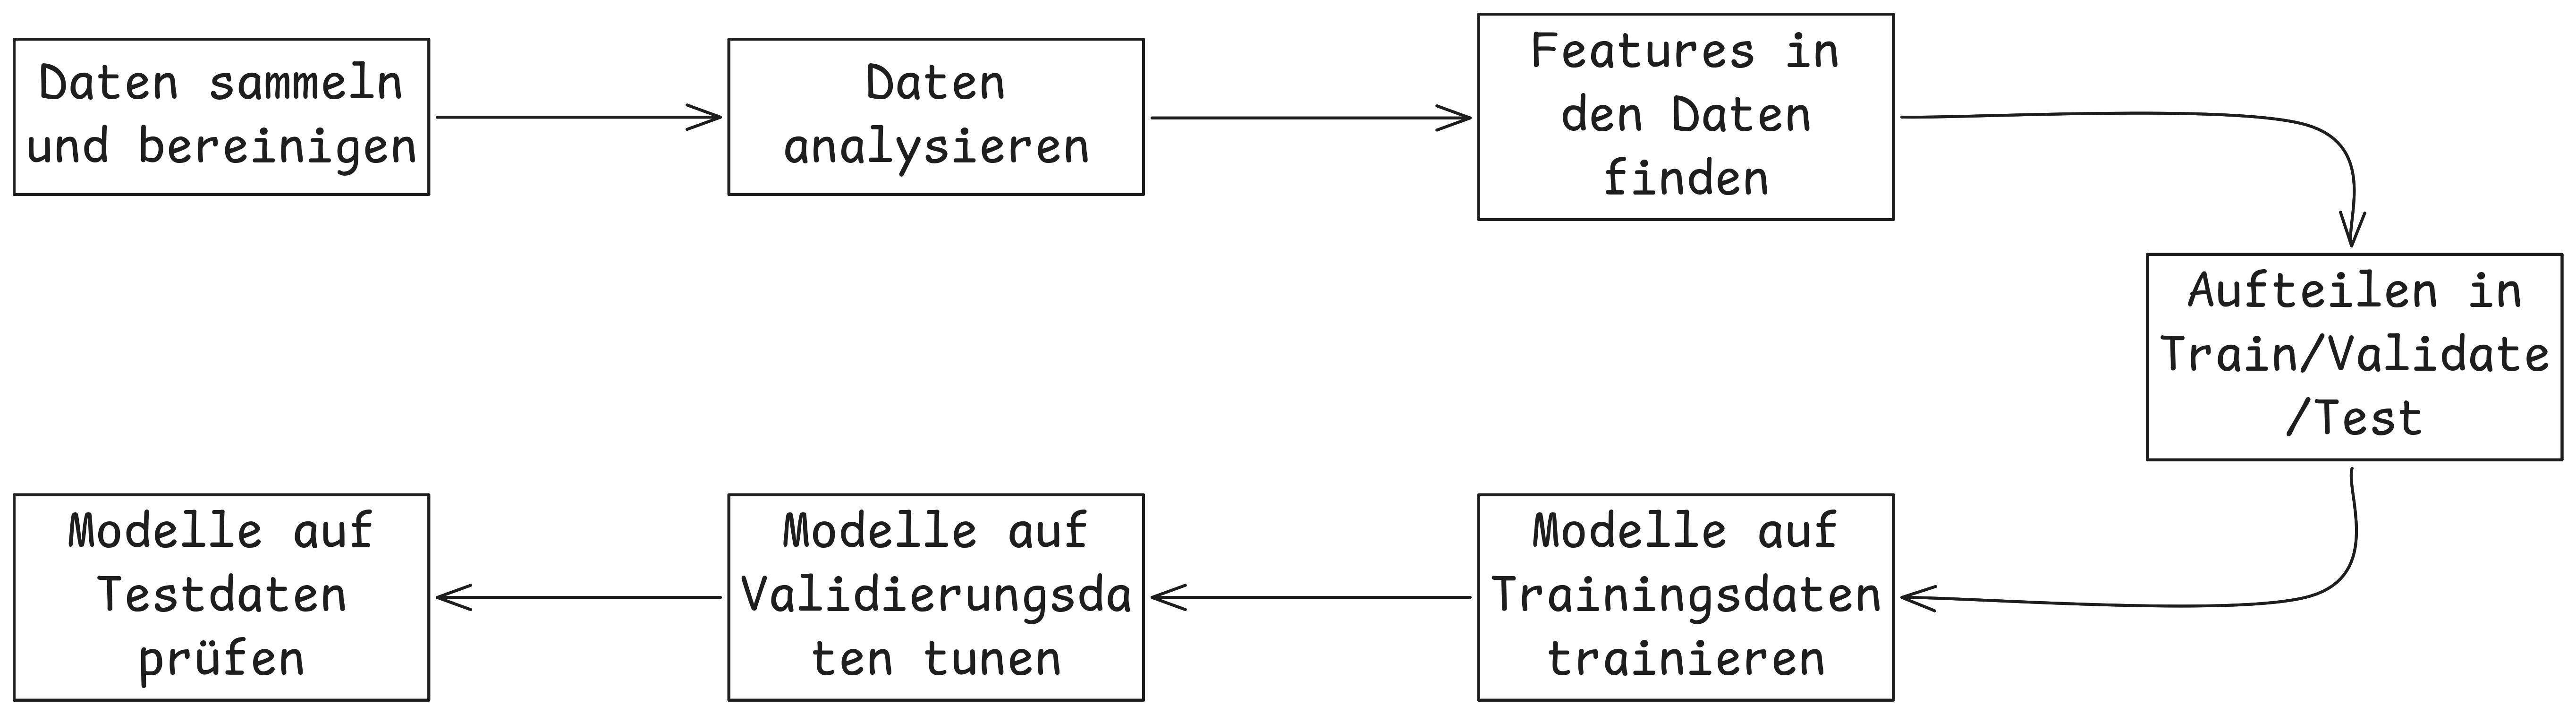
\includegraphics[width=0.9\linewidth]{./img/model_pipeline.png}
	\caption{Machinelerning Modell Pipeline}
    \label{fig:verticalcell}
\end{figure}

\begin{itemize}
    \item Zuerst müssen möglichst viele Relevante Datensätzen gesammelt werden.
	    Dazu gehöhren natürlich historische Aluminium Preis Daten, aber auch historische Preisdaten anderer Metalle.
		Auch Daten die die Wirtschaftliche gesamtlage abbilden, wie bespielsweise der S\&P 500 können relevant sein und werden in die Datenbasis mit aufgenommen.
	\item Diese Daten müssen daraufhin analysiert und bereinigt werden.
		Für eien erste analyse werden sie geplottet und visuel ausgewertet.
		Dabei können vielleicht schon erste Besonderheiten auffallen.
	
	\item im nächsten Schritt werden die Daten dann Maschinell analysiert und Markannte Verknüpfungen (sogenannte Features) unter den Daten können gefunden werden.


	\item um das Vorhersage Modell am Ende auch auf Korrekheit überprüfen zu können werden die Daten in 3 Teile aufgeteilt

	\begin{itemize}
		\item Trainings Daten werden genutzt um das Modell zu Trainieren
		\item Valididerungs Daten werden genutzt um Hyperparamenter des Modells feinzujustieren
		\item Test Daten werden genutzt um das Modell final auf Korrekheit zu überprüfen.
	\end{itemize}

	\item Die daten sind nun vorbereitet und verschiedene Modelle könen trainiert und miteinander verglichen werden.
\end{itemize}


TODO: Aluminium preis historisch Plotten
